\subsection{Current sensor} \label{current_sensor}

The current along with the voltage of the PV allows the system to perform power calculation, which is needed for the MPPT algorithm. The current will be measured in parallel with the inductor with a hall effect sensor. Placing it in series with the PV module would be the easiest approach for MPPT, but placing it in parallel with the inductor allows implementing a current controller for possible future use.

\begin{figure}[htbp]
	\begin{center}
		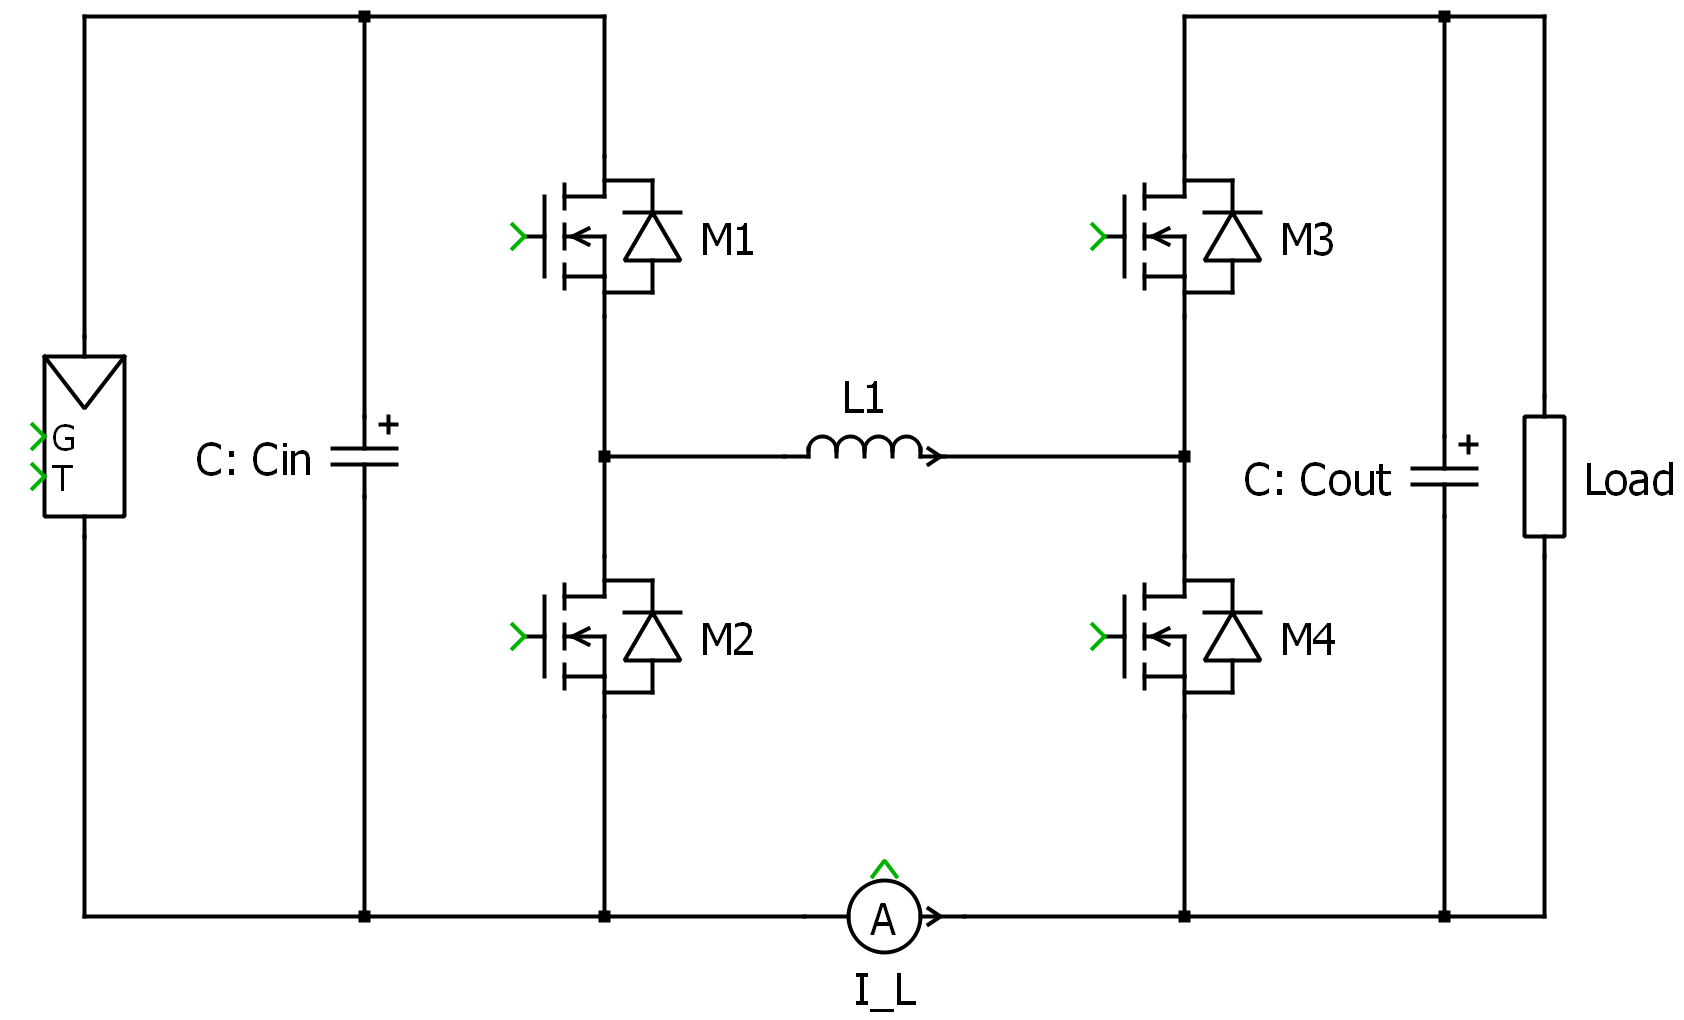
\includegraphics[width=0.4\textwidth]{../Pictures/current_sensor_placement.png}
		\caption{Current sensor placement.}
		\label{current_sensor_placement}
	\end{center}	
\end{figure}

The sensor is a ACS723-20AB which is a Hall effect sensor capable of measuring $\pm 20 A$. It's powered using the $5 V$ bus and has a selectable bandwidth of $20 kHz$ or $80 kHz$. The output of the sensor is a voltage proportional to the current following the next equation:

\begin{equation} 
V_{current} = \frac{1}{8} \, i + 2.5
\end{equation} \todo[inline,color=green]{maybe the gain is 0.1, to be confirmed by test.}

In order to ease the task of the control, the signals are filtered by hardware. The current will be used by the MPPT, which frequency is $100 Hz$ \todo{check final implementation}. The sensor output is filtered by a LPF which cut-off frequency is $500 Hz$. The cut-off frequency has been calculated by a hundredth of the switching frequency, which is $50 kHz$. Also the current might be used in the current controller, this signal will be filtered at $100 KHz$ in order to remove high frequency noise. The filters are first order low-pass filters implemented with a resistor in series with a capacitor.\todo{has the current control been implemented? was enough this filtering?}

In order to calculate the current from the PV module, the converter working mode will have to be taken into account. Assuming continuous conduction mode, the average PV current is:


\begin{equation} 
	Buck \; mode \rightarrow \overline{I_{in}} = i_{measured} \cdot \delta
\end{equation}
\begin{equation} 
Boost \; mode \rightarrow \overline{I_{in}} = i_{measured} \cdot
\end{equation}
\begin{equation} 
Buck-Boost \; mode \rightarrow \overline{I_{in}} = i_{measured} \cdot \delta
\end{equation}

The IC has been placed far from the inductor in order to avoid undesired magnetic flux.

\todo[inline,color=green]{To be written later}